\chapter{Specifikacija programske potpore}
		
	\section{Funkcionalni zahtjevi}
			
			\textbf{\textit{dio 1. revizije}}\\
			
			\textit{Navesti \textbf{dionike} koji imaju \textbf{interes u ovom sustavu} ili  \textbf{su nositelji odgovornosti}. To su prije svega korisnici, ali i administratori sustava, naručitelji, razvojni tim.}\\
				
			\textit{Navesti \textbf{aktore} koji izravno \textbf{koriste} ili \textbf{komuniciraju sa sustavom}. Oni mogu imati inicijatorsku ulogu, tj. započinju određene procese u sustavu ili samo sudioničku ulogu, tj. obavljaju određeni posao. Za svakog aktora navesti funkcionalne zahtjeve koji se na njega odnose.}\\
			
			
			\noindent \textbf{Dionici:}
			
			\begin{packed_enum}
				
				\item Asistent (Naručitelj)
				\item Korisnici				
				\item Vlasnici parkinga
				\item Administrator(i)
				\item Razvojni tim
				
			\end{packed_enum}
			
			\noindent \textbf{Aktori i njihovi funkcionalni zahtjevi:}
			
			
			\begin{packed_enum}
				\item  \underbar{Vlasnik parkinga (inicijator) može:}
				
				\begin{packed_enum}
					
					\item Napraviti (max 1) parkiralište, te ga izbrisati, ili promijeniti ime i cjenik
					\item Ucrtati nova i izbrisati postojeća parking mjesta za svoj parking
					\item Definirati i promijeniti mogućnost rezervacije pojedinog parkirališnog mjesta
					\item Pregledati svoje osobne podatke i promijeniti ih
					\item Izbrisati svoj korisnički račun
					\item Pregledati statistiku zauzetosti svog parkirališta i parkirališnih mjesta kroz vrijeme u obliku grafa
					
				\end{packed_enum}
			
				\item  \underbar{ Neregistrirani/neprijavljeni korisnik (inicijator) može:}
				
				\begin{packed_enum}
					
					\item Registrirati se kao klijent ili kao vlasnik parkinga
					\item Prijaviti se
					\item Pregledati sva parkirališta i parkirališna mjesta dostupna u aplikaciji
					
				\end{packed_enum}
			
				\item  \underbar{Prijavljeni klijent (inicijator) može:}
				
				\begin{packed_enum}
					
					\item Odjaviti se
					\item Pregledati svoje osobne podatke i promijeniti ih
					\item izbrisati korisnički račun
					\item Pregledati sva parkirališta i parkirališna mjesta dostupna u aplikaciji te njihovu zauzetost u realnom vremenu i rezervati ih
					\item Upisati destinaciju, tip prijevoza i procjenu trajanja parkinga te dobiti mogućnost rezervacije najbližeg parkirališnog mjesta
					\item Uplatiti novac u račun
					\item Pregledati povijest transakcija i rezervacija
					
				\end{packed_enum}
			
				\item  \underbar{Administrator (inicijator) može:}
				
				\begin{packed_enum}
					
					\item Odjaviti se
					\item Izbrisati ili promijeniti korisnički račun bilo kojeg ne-administratorskog korisnika
					\item Pregledati sva parkirališta i parkirališna mjesta dostupna u aplikaciji, te promijeniti njihove podatke
					\item Potvrditi novi račun vlasnika parkirališta
					
				\end{packed_enum}
			
				\item  \underbar{Baza podataka (sudionik):}
				
				\begin{packed_enum}
					
					\item Pohranjuje sve podatke o korisnicima i njihovim ovlastima
					\item Pohranjuje sve podatke o parkiralištima (ime, cjenik)
					\item Pohranjuje sve podatke o parkirališnim mjestima (zauzetost, tip)
					
				\end{packed_enum}
			
				\item  \underbar{Senzor zauzetosti (inicijator):}
				
				\begin{packed_enum}
					
					\item Šalje signal kad se parkirališno mjesto zauzme ili oslobodi
					
				\end{packed_enum}
			\end{packed_enum}
			
			\eject 
			
			
				
			\subsection{Obrasci uporabe}
				
				\subsubsection{Opis obrazaca uporabe}
			
					\noindent \underbar{\textbf{UC1 - Dodavanje parkirališta}}
					\begin{packed_item}
						
						\item \textbf{Glavni sudionik: }\text{Voditelj parkirališta}
						\item  \textbf{Cilj:} \text{Dodavanje parkirališta u bazu podataka}
						\item  \textbf{Sudionici:} \text{Voditelj parkirališta, baza podataka}
						\item  \textbf{Preduvjet:} \text{Korisnik mora imati ulogu voditelja parkinga}
						\item  \textbf{Opis osnovnog tijeka:}
						
						\item[] \begin{packed_enum}
							
							\item \text{Voditelj parkirališta odabire opciju za dodavanje parkinga}							
							\item \text{Voditelj parkirališta unosi informacije o svom parkiralištu}							
							\item \text{Voditelj parkirališta na karti unosi dostupna parkirališna mjesta}							
													
							\item \text{Voditelj parkirališta postavlja senzor koji osvježava informaciju zauzetosti parkirališnog mjesta}						
						\end{packed_enum}
						
						\item  \textbf{Opis mogućih odstupanja:}
						
						\item[] \begin{packed_item}
							
							\item[2.a] Unešeno već postojeće ime parkinga
							\item[] \begin{packed_enum}
								
								\item Aplikacija ispisuje grešku
								
							\end{packed_enum}
							\item[3.a] Označavanje mjesta na karti na kojem već postoji parking
							\item[] \begin{packed_enum}
								
								\item Aplikacija ispisuje grešku
								
							\end{packed_enum}
							\item[4.a] Aplikacija se ne može povezati sa senzorom
							\item[] \begin{packed_enum}
								
								\item Aplikacija ispisuje grešku
								
							\end{packed_enum}
							
						\end{packed_item}
					\end{packed_item}
					\noindent \underbar{\textbf{UC2 - Brisanje parkirališta}}
					\begin{packed_item}
						
						\item \textbf{Glavni sudionik: }Voditelj parkirališta
						\item  \textbf{Cilj:} Brisanje parkirališta
						\item  \textbf{Sudionici:} Voditelj parkirališta, baza podataka
						\item  \textbf{Preduvjet:} Korisnik mora imati ulogu voditelja parkinga, voditelj mora upravljati tim parkingom, parkiralište već postoji u bazi podataka
						\item  \textbf{Opis osnovnog tijeka:}
						
						\item[] \begin{packed_enum}
							
							
							\item Voditelj zatraži brisanje parkirališta
							\item Parkiralište se briše iz baze podataka
							\item Voditelju se javlja da je parkiralište uspješno izbrisano
							
						\end{packed_enum}
						
						\item  \textbf{Opis mogućih odstupanja:}
						
						\item[] \begin{packed_item}
							
							\item[2.a] Neuspješno brisanje podataka iz baze podataka	
							\item[] \begin{packed_enum}
								
								\item Aplikacija ispisuje grešku
								
							\end{packed_enum}
						\end{packed_item}
					\end{packed_item}
				    \noindent \underbar{\textbf{UC3 - Izmjena podataka o parkiralištu}}
				   \begin{packed_item}
				   	
				   	\item \textbf{Glavni sudionik: }Voditelj parkirališta
				   	\item  \textbf{Cilj:} Izmjena podataka o parkiralištu
				   	\item  \textbf{Sudionici:} Voditelj parkirališta, baza podataka
				   	\item  \textbf{Preduvjet:} Korisnik mora imati ulogu voditelja parkinga, voditelj mora upravljati tim parkingom, parkiralište već postoji u bazi podataka
				   	\item  \textbf{Opis osnovnog tijeka:}
				   	
				   	\item[] \begin{packed_enum}
				   		
				   		\item Voditelj zatraži izmjenu podataka
				   		\item Voditelj unosi nove izmjenjene podatke o parkiralištu
				   		\item Novi podatci se spremaju u bazu podataka
				   		\item Voditelju se javlja da su podatci uspješno izmjenjeni
				   	\end{packed_enum}
				   	
				   	\item  \textbf{Opis mogućih odstupanja:}
				   	
				   	\item[] \begin{packed_item}
				   		
				   		
				   		
				   		\item[3.a] Neuspješno spremanje podataka u bazu podataka	
				   		\item[] \begin{packed_enum}
				   			
				   			\item Aplikacija ispisuje grešku
				   			
				   		\end{packed_enum}
				   		
				   	\end{packed_item}
				   \end{packed_item}
			    	\noindent \underbar{\textbf{UC4 - Izmjena podataka o parkirališnom mjestu}}
			    	\begin{packed_item}
			    		
			    		\item \textbf{Glavni sudionik: }Voditelj parkirališta
			    		\item  \textbf{Cilj:} Izmjena podataka o parkirališnom mjestu
			    		\item  \textbf{Sudionici:} Voditelj parkirališta, baza podataka
			    		\item  \textbf{Preduvjet:} Korisnik mora imati ulogu voditelja parkinga, voditelj mora upravljati tim parkingom, parkiralište i parkirno mjesto već postoji u bazi podataka
			    		\item  \textbf{Opis osnovnog tijeka:}
			    		
			    		\item[] \begin{packed_enum}
			    			
			    			\item Voditelj zatraži izmjenu podataka
			    			\item Voditelj unosi nove izmjenjene podatke o parkirališnom mjestu
			    			\item Novi podatci se spremaju u bazu podataka
			    			\item Voditelju se javlja da su podatci uspješno izmjenjeni
			    		\end{packed_enum}
			    		
			    		\item  \textbf{Opis mogućih odstupanja:}
			    		
			    		\item[] \begin{packed_item}
			    			\item[3.a] Neuspješno spremanje podataka u bazu podataka	
			    			\item[] \begin{packed_enum}
			    				
			    				\item Aplikacija ispisuje grešku
			    				
			    			\end{packed_enum}
			    			
			    	\end{packed_item}
		    		\noindent \underbar{\textbf{UC5 - Dodavanje parkirališnog mjesta}}
		    		\begin{packed_item}
		    			\item \textbf{Glavni sudionik: }Voditelj parkirališta
		    			\item  \textbf{Cilj:} Dodavanje parkirališnog mjesta
		    			\item  \textbf{Sudionici:} Voditelj parkirališta, baza podataka
		    			\item  \textbf{Preduvjet:} Korisnik mora imati ulogu voditelja parkinga, voditelj mora upravljati tim parkingom, parkiralište i parkirno mjesto već postoji u bazi podataka
		    			\item  \textbf{Opis osnovnog tijeka:}
		    			
		    			\item[] \begin{packed_enum}
		    				
		    				\item Voditelj zatraži dodavanje novog parkirališnog mjesta na parkiralištu
		    				\item Voditelj na karti ucrtaje parkirališno mjesto
		    				\item Voditelj parkirališta definira je li moguće rezervirati parkirališno mjesto
		    				\item Podatci se spremaju u bazu podataka
		    				\item Voditelju se javlja da su podatci uspješno spremljeni u bazi podataka
		    			\end{packed_enum}
		    			
		    			\item  \textbf{Opis mogućih odstupanja:}
		    			
		    			\item[] \begin{packed_item}
		    				
		    				\item[2.a] Voditelj dodaje parkirališno mjesto na lokaciji na kojoj vec postoji parkirališno mjesto
		    				\item[] \begin{packed_enum}
		    					
		    					\item Voditelja se upozorava o grešci
		    					
		    				\end{packed_enum}
	    				
	    				\item[4.a] Neuspješno spremanje podataka u bazu podataka	
	    				\item[] \begin{packed_enum}
	    					
	    					\item Aplikacija ispisuje grešku
	    					
	    				\end{packed_enum}
		    				
		    			\end{packed_item}
		    		\end{packed_item}
	    			\noindent \underbar{\textbf{UC6 - Brisanje parking mjesta}}
	    			\begin{packed_item}
	    				
	    				\item \textbf{Glavni sudionik: }Voditelj parkirališta
	    				\item  \textbf{Cilj:} Brisanje parking mjesta
	    				\item  \textbf{Sudionici:} Voditelj parkirališta, baza podataka
	    				\item  \textbf{Preduvjet:} Korisnik mora imati ulogu voditelja parkinga, voditelj mora upravljati tim parkingom, parkiralište već postoji u bazi podataka
	    				\item  \textbf{Opis osnovnog tijeka:}
	    				
	    				\item[] \begin{packed_enum}
	    					
	    					\item Voditelj zatraži brisanje parkiraling mjesta
	    					\item Parkirališno mjesto se briše iz baze podataka
	    					\item Voditelju se javlja da je parkiralište uspješno izbrisano
	    				\end{packed_enum}
	    				
	    				\item  \textbf{Opis mogućih odstupanja:}
	    				
	    				\item[] \begin{packed_item}
	    					
	    					\item[2.a] Neuspješno brisanje podataka iz baze podataka	
	    					\item[] \begin{packed_enum}
	    						
	    						\item Aplikacija ispisuje grešku
	    						
	    					\end{packed_enum}
	    				\end{packed_item}
	    			\end{packed_item}
    				\noindent \underbar{\textbf{UC7 - Definiranje mogućnosti rezervacije pojedinog parkirališnog mjesta}}
    				\begin{packed_item}
    					
    					\item \textbf{Glavni sudionik: }Voditelj parkirališta
    					\item  \textbf{Cilj:} Definiranje mogućnosti rezervacije pojedinog parkirališnog mjesta
    					\item  \textbf{Sudionici:} Voditelj parkirališta, baza podataka
    					\item  \textbf{Preduvjet:} Korisnik mora imati ulogu voditelja parkinga, voditelj mora upravljati tim parkingom, parkiralište već postoji u bazi podataka
    					\item  \textbf{Opis osnovnog tijeka:}
    					
    					\item[] \begin{packed_enum}
    						
    						\item Voditelj odabire parkirališno mjesto 
    						\item Voditelj definira mogućnost rezervacije parkirališnog mjesta
    						\item Informacije se spremaju u bazi podataka
    						\item Voditelju se javlja da su podatci uspješno spremljeni
    					
    					\end{packed_enum}
    					
    					\item  \textbf{Opis mogućih odstupanja:}
    					
    					\item[] \begin{packed_item}
    						
    						\item[3.a] Neuspješno spremanje podataka u bazu podataka	
    						\item[] \begin{packed_enum}
    							
    							\item Aplikacija ispisuje grešku
    							
    						\end{packed_enum}
    						
    					\end{packed_item}
    				\end{packed_item}
    				\noindent \underbar{\textbf{UC8 - Promjena mogućnosti rezervacije pojedinog parkirališnog mjesta}}
    				\begin{packed_item}
    					
    					\item \textbf{Glavni sudionik:} Senzor zauzetosti
    					\item  \textbf{Cilj:} Omogućuje ponovnu rezervaciju novog tek oslobođenog mjesta
    					\item  \textbf{Sudionici:} Baza podataka
    					\item  \textbf{Preduvjet:} 
    					\item  \textbf{Opis osnovnog tijeka:}
    					
    					\item[] \begin{packed_enum}
    						
    						\item Vozilo dođe ili ode sa parkirališnog mjesta
    						\item Senzor registrira promjenu
    						\item Promjena se pohranjuje u bazu podataka
    					\end{packed_enum}
    					
    					\item  \textbf{Opis mogućih odstupanja:}
    					
    					\item[] \begin{packed_item}
    						
    						\item[2.a] Kvar na senzoru zauzetosti
    						\item[] \begin{packed_enum}
    							
    							\item Hitan popravak ili zamjena senzora od strane vlasnika parkinga
    							
    						\end{packed_enum}
    						
    					\end{packed_item}
    				\end{packed_item}
    			
    				\noindent \underbar{\textbf{UC9 - Pregled osobnih podataka}}
    				\begin{packed_item}
    					
    					\item \textbf{Glavni sudionik:} Administrator
    					\item  \textbf{Cilj:} Dati administratoru posebnu mogućnost pregleda osobnih podataka svih registriranih korisnika
    					\item  \textbf{Sudionici:} Baza podataka
    					\item  \textbf{Preduvjet:} Glavni sudionik nužno mora biti prijavljen kao administrator
    					\item  \textbf{Opis osnovnog tijeka:}
    					
    					\item[] \begin{packed_enum}
    						
    						\item Administrator zatraži pregled osobnih podataka određenog registriranog korisnika
    						\item Određeni podaci se dohvaćaju iz baze podataka
    						\item Podaci se formatirano prikazuju administratoru
    					\end{packed_enum}
    					
    					\item  \textbf{Opis mogućih odstupanja:}
    					
    					\item[] \begin{packed_item}
    						
    						\item[2.a] Neuspjelo dohvaćanje podataka iz baze podataka
    						\item[] \begin{packed_enum}
    							
    							\item Aplikacija ispisuje grešku
    							
    						\end{packed_enum}
    						
    					\end{packed_item}
    				\end{packed_item}
    				\noindent \underbar{\textbf{UC10 - Promjena osobnih podataka}}
    				\begin{packed_item}
    					
    					\item \textbf{Glavni sudionik:} Administrator
    					\item  \textbf{Cilj:} Dati administratoru posebnu mogućnost izmjene osobnih podataka svih registriranih korisnika
    					\item  \textbf{Sudionici:} Baza podataka
    					\item  \textbf{Preduvjet:} Glavni sudionik nužno mora biti prijavljen kao administrator
    					\item  \textbf{Opis osnovnog tijeka:}
    					
    					\item[] \begin{packed_enum}
    						
    						\item Administrator zatraži pregled osobnih podataka određenog registriranog korisnika
    						\item Određeni podaci se dohvaćaju iz baze podataka
    						\item Administrator odluči mijenjati osobne podatke odabranog korisnika
    						\item Administrator potvrdi promjene
    						\item Promjene se pohranjuju u bazu podataka
    					\end{packed_enum}
    					
    					\item  \textbf{Opis mogućih odstupanja:}
    					
    					\item[] \begin{packed_item}
    						
    						\item[2.a] Neuspjelo dohvaćanje podataka iz baze podataka
    						\item[] \begin{packed_enum}
    							
    							\item Aplikacija ispisuje grešku
    							
    						\end{packed_enum}
    						\item[3.a] Administrator je unio krivi format podataka
    						\item[] \begin{packed_enum}
    							
    							\item Aplikacija upozorava na krivi format i ne dopušta potvrdu
    							
    						\end{packed_enum}
    						\item[5.a] Neuspjela pohrana u bazu podataka
    						\item[] \begin{packed_enum}
    							
    							\item Aplikacija ispisuje grešku
    							
    						\end{packed_enum}
    						
    					\end{packed_item}
    				\end{packed_item}
    				\noindent \underbar{\textbf{UC11 - Registracija u sustav}}
    			\begin{packed_item}
    				
    				\item \textbf{Glavni sudionik:} Neregistrirani korisnik 
    				\item  \textbf{Cilj:} Omogućuje neregistriranom korisniku registraciju u sustav
    				\item  \textbf{Sudionici:} Baza podataka
    				\item  \textbf{Preduvjet:} Glavni sudionik nije registriran od prije
    				\item  \textbf{Opis osnovnog tijeka:}
    				
    				\item[] \begin{packed_enum}
    					
    					\item Neregistrirani korisnik šalje zahtjev za registraciju sa određenom ulogom za koju se hoće prijaviti (voditelj parkinga ili klijent)
    					\item Neregistrirani korisnik upisuje potrebne podatke (ime, prezime email,...)
    					\item Neregistrirani korisnik potvrđuje svoje podatke
    					\item Ako se korisnik prijavio kao voditelj parkinga administrator ga mora potvrditi
    					\item Podaci o novoregistriranom korisniku se pohranjuju u bazu podataka
    					\item Registracija se završava potvrdom preko email adrese
    				\end{packed_enum}
    				
    				\item  \textbf{Opis mogućih odstupanja:}
    				
    				\item[] \begin{packed_item}
    					
    					\item[2.a] Upisani podaci nisu u pravilnom formatu
    					\item[] \begin{packed_enum}
    						
    						\item Aplikacija upozorava na krivi format i ne dopušta nastavak
    						
    					\end{packed_enum}
    					\item[5.a] Neuspjela pohrana u bazu podataka
    					\item[] \begin{packed_enum}
    						
    						\item Aplikacija dojavljuje grešku i ne dopušta nastavak
    						
    					\end{packed_enum}
    					
    				\end{packed_item}
    			\end{packed_item}
    				\noindent \underbar{\textbf{UC12 - Prijava u sustav}}
    			\begin{packed_item}
    				
    				\item \textbf{Glavni sudionik:} Bilo koji registrirani korisnik (klijent, vlasnik, admin)
    				\item  \textbf{Cilj:} Dobiti pristup korisničkom sučelju  
    				\item  \textbf{Sudionici:} Baza podataka
    				\item  \textbf{Preduvjet:} Korisnik je već registriran u sustav
    				\item  \textbf{Opis osnovnog tijeka:}
    				
    				\item[] \begin{packed_enum}
    					
    					\item Korisnik unosi korisničko ime i lozinku
    					\item Provjerava se postoje li upisani podaci u bazi podataka
    					\item Korisnik dobiva pristup korisničkim funkcijama
    				\end{packed_enum}
    				
    				\item  \textbf{Opis mogućih odstupanja:}
    				
    				\item[] \begin{packed_item}
    					
    					\item[2.a] Upisano korisničko i lozinka su netočni
    					\item[] \begin{packed_enum}
    						
    						\item Sustav obavještava korisnika o neispravnom upisu
						\end{packed_enum}
    					
    				\end{packed_item}
    			\end{packed_item}
    				\noindent \underbar{\textbf{UC13 - Odjava iz sustava}}
    				\begin{packed_item}
    					
    					\item \textbf{Glavni sudionik:} Bilo koji registrirani korisnik (klijent, vlasnik, admin) 
    					\item  \textbf{Cilj:} Odjavljivanje iz korisničkog sučelja
    					\item  \textbf{Sudionici:} 
    					\item  \textbf{Preduvjet:} Korisnik prijavljen u sustav
    					\item  \textbf{Opis osnovnog tijeka:}
    					
    					\item[] \begin{packed_enum}
    						
    						\item Korisnik zatraži odjavu iz sustava
    						\item Korisnik izlazi iz korisničkog sučelja
   
    					\end{packed_enum}
    					
    				\end{packed_item}
    				\noindent \underbar{\textbf{UC14 - Brisanje korisničkog računa}}
    			\begin{packed_item}
    				
    				\item \textbf{Glavni sudionik:} Bilo koji registrirani korisnik (klijent, vlasnik, admin) 
    				\item  \textbf{Cilj:} Omogućuje brisanje korisničkog računa
    				\item  \textbf{Sudionici:} Baza podataka
    				\item  \textbf{Preduvjet:} Korisnik je prijavljen u sustav
    				\item  \textbf{Opis osnovnog tijeka:}
    				
    				\item[] \begin{packed_enum}
    					
    					\item Korisnik zatraži brisanje korisničkog računa
    					\item Korisničko ime i lozinka korisnika se brišu iz baze podataka
    					\item Izlazak iz korisničkog sučelja
    				\end{packed_enum}
    				

    			\end{packed_item}
    				\noindent \underbar{\textbf{UC15 - Pregled statistike zauzetosti}}
    				\begin{packed_item}
    					
    					\item \textbf{Glavni sudionik:} Voditelj
    					\item  \textbf{Cilj:} Voditelj može voditi evidenciju o zauzetosti svojih parkirališnih mjesta
    					\item  \textbf{Sudionici:} Baza podataka
    					\item  \textbf{Preduvjet:} Korisnik je prijavljen kao voditelj
    					\item  \textbf{Opis osnovnog tijeka:}
    					
    					\item[] \begin{packed_enum}
    						
    						\item Voditelj odluči vidjeti zauzetost svih svojih parkirališnim mjesta
    						\item Dohvaćanje podataka o zauzetosti iz baze podataka
    						\item Voditelj pregledava podatke te donosi daljnje odluke
    					\end{packed_enum}
    					
    					\item  \textbf{Opis mogućih odstupanja:}
    					
    					\item[] \begin{packed_item}
    						
    						\item[2.a] Nema nijedno parkirno mjesto
    						\item[] \begin{packed_enum}
    							
    							\item Ispis pogreške
    							\item Voditelju omoguceno dodavanje parkirnih mjesta
    							
    						\end{packed_enum}
    						
    					\end{packed_item}
    				\end{packed_item}
    				\noindent \underbar{\textbf{UC16 - Pregled dostupnih parkirališnih mjesta}}
    				\begin{packed_item}
    					
    					\item \textbf{Glavni sudionik: } Registrirani i neregistrirani korisnici
    					\item  \textbf{Cilj:} Uvid u dostupna parkirališna mjesta
    					\item  \textbf{Sudionici:} Baza podataka
    					\item  \textbf{Preduvjet:} Nema
    					\item  \textbf{Opis osnovnog tijeka:}
    					
    					\item[] \begin{packed_enum}
    						
    						\item Odabir parkinga te parkirališnog mjesta
    						\item Dohvaćanje podataka iz baze podataka
    						\item Daljnje registriranje u slučaju da korisnik želi izvršiti rezervaciju

    					\end{packed_enum}
    					
    					\item  \textbf{Opis mogućih odstupanja:}
    					
    					\item[] \begin{packed_item}
    						
    						\item[2.a] Nema slobodnih parkirališnih mjesta
    						\item[] \begin{packed_enum}
    							
    							\item Poruka o popunjenosti parkinga
    							
    						\end{packed_enum}
    						
    					\end{packed_item}
    				\end{packed_item}
    				\noindent \underbar{\textbf{UC17 - Pregled zauzetosti parkirališnih mjesta}}
    				\begin{packed_item}
    					
    					\item \textbf{Glavni sudionik: } Klijent
    					\item  \textbf{Cilj:} Svaki klijent može evidentirati zauzetost o svim parkirnim mjestima
    					\item  \textbf{Sudionici:} Baza podataka
    					\item  \textbf{Preduvjet:} Korisnik prijavljen kao klijent te postoje parkirna mjesta
    					\item  \textbf{Opis osnovnog tijeka:}
    					
    					\item[] \begin{packed_enum}
    						
    						\item Klijent odluči vidjeti podatke o zauzetosti
    						\item Dohvat svih parkirnih mjesta
    						\item Odabir pojedinog parkirnog mjesta
    						\item Dohvat podataka iz baze podataka
    						\item Uvid u dostavljene podatke 
    					\end{packed_enum}
    					
    					\item  \textbf{Opis mogućih odstupanja:}
    					
    					\item[] \begin{packed_item}
    						
    						\item[2.a] Nema nijedno parkirno mjesto
    						\item[] \begin{packed_enum}
    							
    							\item Poruka 
    							
    						\end{packed_enum}
    						
    					\end{packed_item}
    				\end{packed_item}
    				\noindent \underbar{\textbf{UC18 - Rezervacija parkirališnog mjesta}}
    				\begin{packed_item}
    					
    					\item \textbf{Glavni sudionik: } Klijent
    					\item  \textbf{Cilj:} Klijent rezervira parkirališno mjesto
    					\item  \textbf{Sudionici:} Baza podataka
    					\item  \textbf{Preduvjet:} Korisnik rezerviran kao klijent
    					\item  \textbf{Opis osnovnog tijeka:}
    					
    					\item[] \begin{packed_enum}
    						
    						\item Korisnik odluči rezervirati parkirno mjesto
    						\item Otvaranje karte te odabir tipa prijevoza te trajanje parkinga	
    						\item Iscrtavanje rute do najbliže slobodnog parkirališnog mjesta
    						\item Klijent odabire jedan od 2 načina rezerviranja
    						\item Nastavak na plaćanje
    					\end{packed_enum}
    					
    					\item  \textbf{Opis mogućih odstupanja:}
    					
    					\item[] \begin{packed_item}
    						
    						\item[3.a] Nema slobodnih parkirališnih mjesta
    						\item[] \begin{packed_enum}
    							
    							\item Ispis pogreške
    							\item Preusmjeravanje nazad na ispunjavanje obrasca o traženju slobodnih parkirnih mjesta
    							
    						\end{packed_enum}
    						
    						
    					\end{packed_item}
    				\end{packed_item}
    				\noindent \underbar{\textbf{UC19 - Upis destinacije, tipa prijevoza i procjene trajanja parkinga}}
    				\begin{packed_item}
    					
    					\item \textbf{Glavni sudionik: } Klijent
    					\item  \textbf{Cilj:} Unos podataka za rezervaciju parkinga
    					\item  \textbf{Sudionici:} Baza podataka
    					\item  \textbf{Preduvjet:} Korisnik registriran kao klijent
    					\item  \textbf{Opis osnovnog tijeka:}
    					
    					\item[] \begin{packed_enum}
    						
    						\item Upis destinacije, tipa prijevoza i procjene trajanja parkinga
    						\item Filtriranje slobodnih parkirnih mjesta
    						\item Rezervacija parkirnog mjesta

    					\end{packed_enum}
    					
    					\item  \textbf{Opis mogućih odstupanja:}
    					
    					\item[] \begin{packed_item}
    						
    						\item[2.a] Unos krivih podataka
    						\item[] \begin{packed_enum}
    							
    							\item Poruka te ponovna mogućnost unosa podataka
    					
    						\end{packed_enum}
    						
    					\end{packed_item}
    				\end{packed_item}
    				\noindent \underbar{\textbf{UC20 - Uplata novca na račun}}
    			\begin{packed_item}
    				
    				\item \textbf{Glavni sudionik: } Klijent
    				\item  \textbf{Cilj:} Uplata klijenta na račun vlasnika parkinga
    				\item  \textbf{Sudionici:} Baza podataka, Vlasnik parkinga
    				\item  \textbf{Preduvjet:} Korisnik registriran kao klijent te klijent izvršio rezervaciju
    				\item  \textbf{Opis osnovnog tijeka:}
    				
    				\item[] \begin{packed_enum}
    					
    					\item Uvid u cijenu željenog parkirališnog mjesta
    					\item Klijent dodaje novac u novčanik
    					\item Klijent plaća novac na voditeljeov račun
    					\item Ažuriranje novčanika u bazi podataka
    					\item Potvrda o uspješnoj transakciji

    				\end{packed_enum}
    				
    				\item  \textbf{Opis mogućih odstupanja:}
    				
    				\item[] \begin{packed_item}
    					
    					\item[2.a] Klijent nema dovoljno novca u novčaniku
    					\item[] \begin{packed_enum}
    						
    						\item Ispis poruke
    						\item Preusmjeravanje na dodavanje novca u novčanik
    						
    					\end{packed_enum}
    					\item[3.a] Neuspjelo ažuriranje podataka
						\item[] \begin{packed_enum}
							
							\item Ispis poruke
							\item Preusmjeravanje na ponovno izvršavanje transakcije
							
						\end{packed_enum}
    					
    				\end{packed_item}
    			\end{packed_item}
    				\noindent \underbar{\textbf{UC21 -Pregled povijesti transakcija i rezervacija}}
    				\begin{packed_item}
    					
    					\item \textbf{Glavni sudionik: }Voditelj parkirališta
    					\item  \textbf{Cilj:}Pregled povijesti transakcija i rezervacija 
    					\item  \textbf{Sudionici:} Voditelj parkirališta i baza podataka
    					\item  \textbf{Preduvjet:} Korisnik mora imati ulogu voditelja parkinga, voditelj mora upravljati tim parkingom, parkiralište već postoji u bazi podataka
    					\item  \textbf{Opis osnovnog tijeka:}
    					
    					\item[] \begin{packed_enum}
    						
    						\item Voditelj zatraži pregled povijesti transakcija i rezervacija
    						\item Podatci se dohvaćaju iz baze podataka
    						\item Podatci se ispisuju voditelju
    						
    					\end{packed_enum}
    					
    					\item  \textbf{Opis mogućih odstupanja:}
    					
    					\item[] \begin{packed_item}
    						
    					\item[2.a] Neuspješno spremanje podataka u bazu podataka	
    					\item[] \begin{packed_enum}
    						
    						\item Aplikacija ispisuje grešku
    						
    					\end{packed_enum}
    						
    					\end{packed_item}
    				\end{packed_item}
    				\noindent \underbar{\textbf{UC22 - Potvrda računa vlasnika}}
    				\begin{packed_item}
    					
    					\item \textbf{Glavni sudionik: } Administrator
    					\item  \textbf{Cilj:} Potvrditi račun voditelja parkinga
    					\item  \textbf{Sudionici:} Baza podataka
    					\item  \textbf{Preduvjet:} Vlasnik je napravio račun potvrdom email adrese te korisnik je prijavljen kao administrator
    					\item  \textbf{Opis osnovnog tijeka:}
    					
    					\item[] \begin{packed_enum}
    						
    						\item Administrator pregledava voditeljev račun
    						\item Odabire funkcionalnost potvrđivanja u slučaju valjanosti računa suprotno odbacuje račun

    					\end{packed_enum}
    					
    					\item  \textbf{Opis mogućih odstupanja:}
    					
    					
    				\end{packed_item}
    				
				
					
				\subsubsection{Dijagrami obrazaca uporabe}
					
					\begin{figure}[H]

						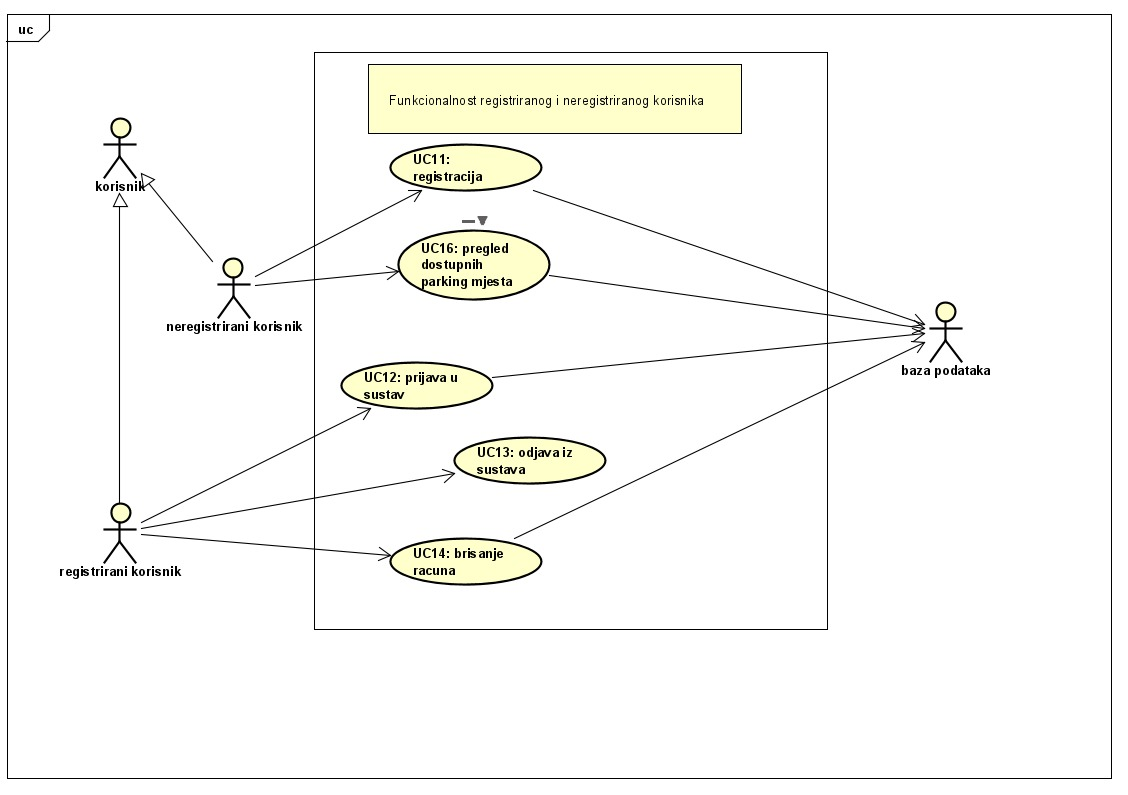
\includegraphics[width=\textwidth]{slika.jpeg} %veličina slike u odnosu na originalnu datoteku i pozicija slike
						\centering
						\caption{UC registrirani i neregistrirani korisnik}
						\label{fig:registrirani4312}
					\end{figure}
					
                    \begin{figure}[H]
						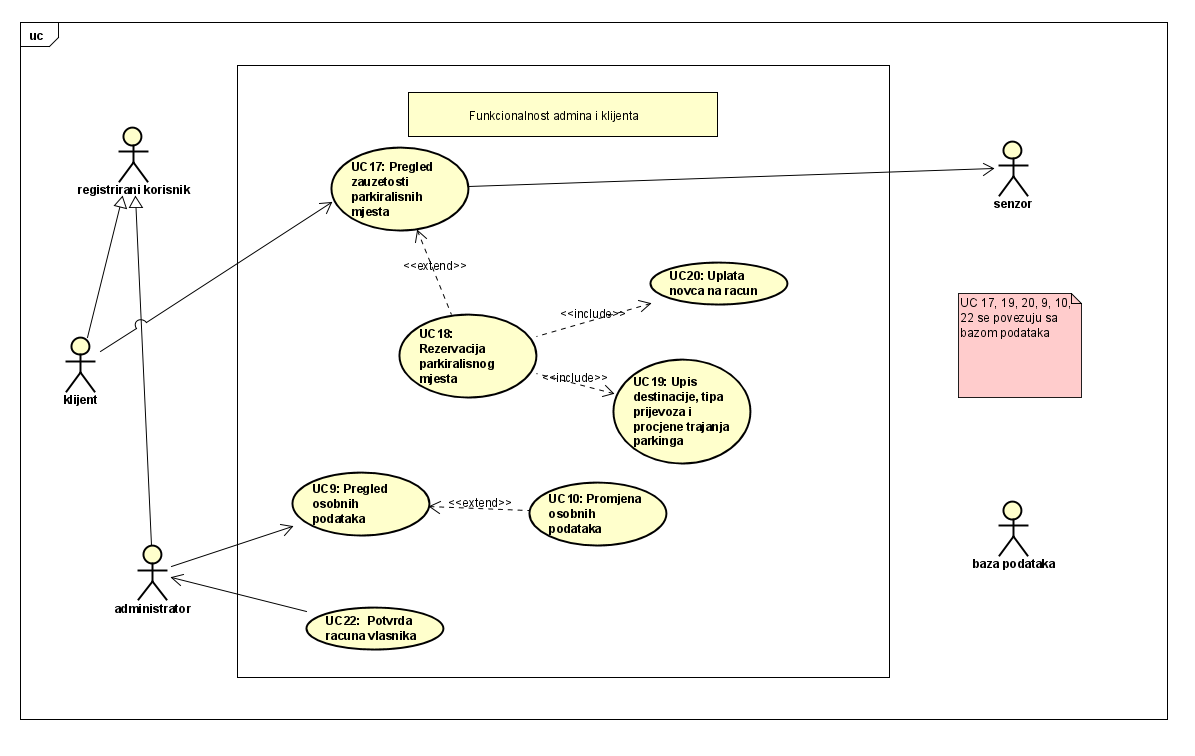
\includegraphics[width=\textwidth]{slike/klijent.PNG} %veličina slike u odnosu na originalnu datoteku i pozicija slike
						\caption{UC funkcionalnost klijenta i administratora}
						\label{fig:klijent}
					\end{figure}
				
				   \begin{figure}[H]
				   	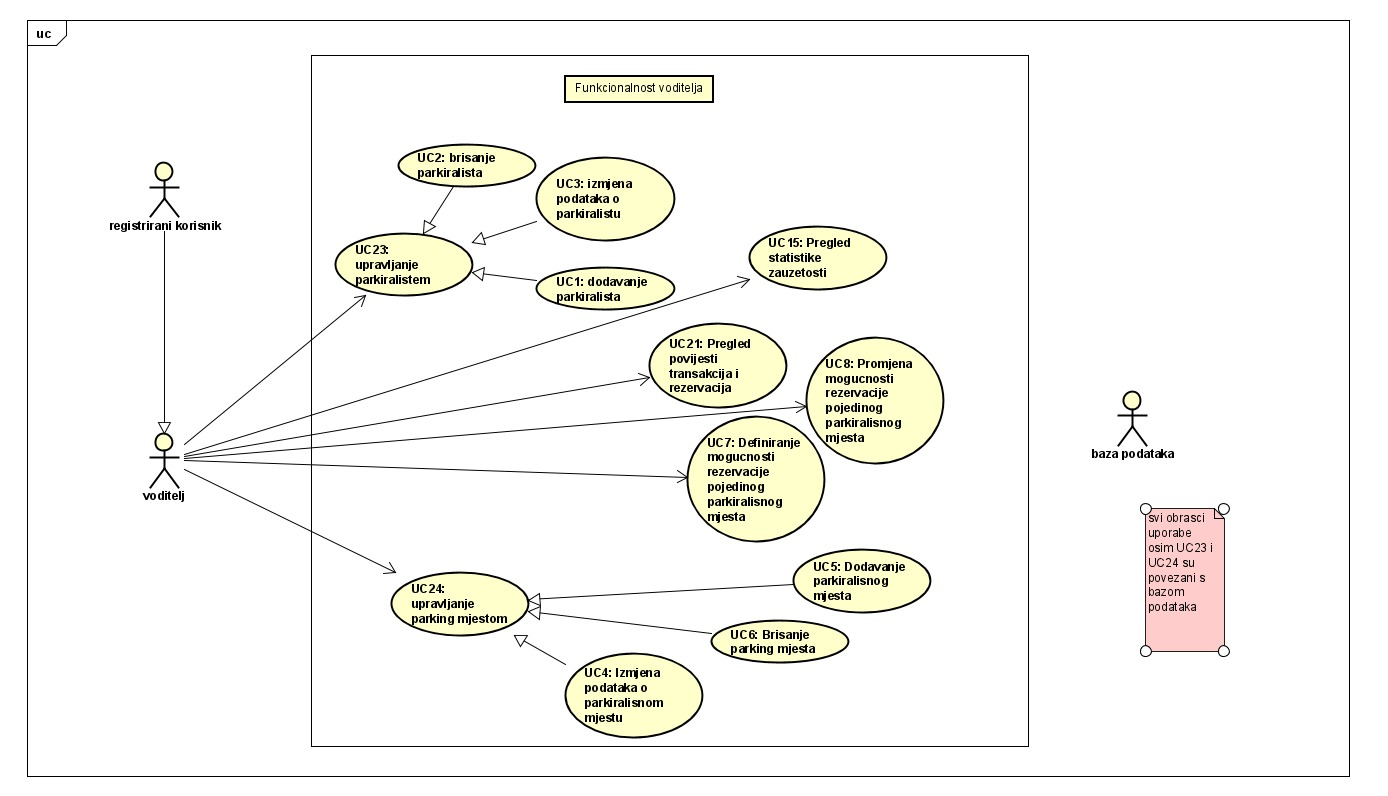
\includegraphics[width=\textwidth]{slike/Voditelj.jpeg} %veličina slike u odnosu na originalnu datoteku i pozicija slike
				   	\caption{UC funkcionalnost voditelja}
				   	\label{fig:voditelj}
				   \end{figure}
				\eject		

				
			\subsection{Sekvencijski dijagrami}
				
				\textbf{Obrazac uporabe UC18 - Rezervacija parkirališnog mjesta}\\
				
				Klijent odabire svoje odredište, tip prijevoza i procjenu trajanja parkinga. Aplikacija mu pronalazi najbliži parking te prikazuje njegovu zauzetost. Klijent sada ima dvije mogućnosti: prvo odabrati termin nakon čega mu aplikacija dohvaća iz baze podataka slobodna mjesta u tom terminu ili najprije odabrati parking mjesto nakon čega mu aplikacija dohvaća iz baze podataka slobodne termine za to mjesto. Nakon klijentovog odabira aplikacija izračunava cijenu parkinga. U ovom slučaju uzeli smo opciju da klijent plaća putem aplikacije. Nakon plaćanja rezervacija se pohranjuje u bazu podataka i ispisuje se potvrda o rezervaciji. Postupak je iterativan. 
				\eject	
						
			 	\begin{figure}[H]
					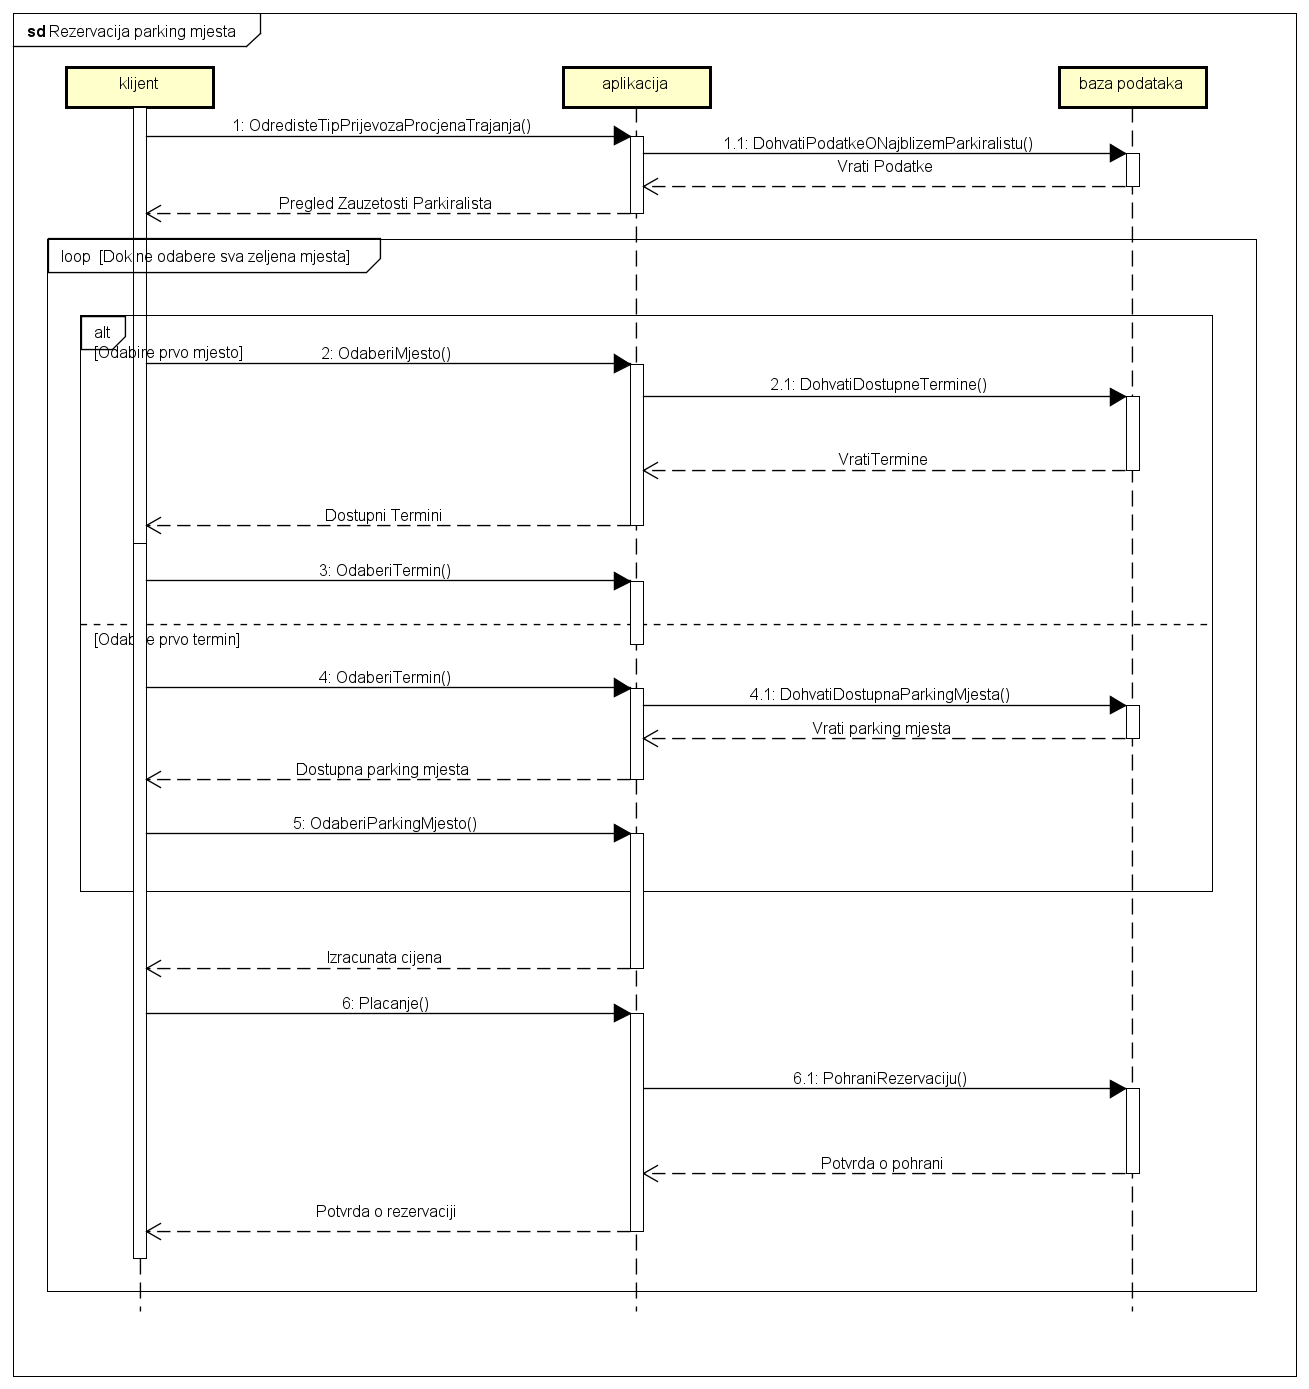
\includegraphics[width=\textwidth]{slike/RezervacijaParkingMjesta.png} %veličina slike u odnosu na originalnu datoteku i pozicija slike
					\caption{Sekvencijski dijagram za UC18}
					\label{fig:rezarvacija}
				\end{figure}
				\eject	
				
				\textbf{Obrazac uporabe UC7 - Definiranje mogućnosti rezervacije pojedinog parkirališnog mjesta}\\
				
				Voditelj zatraži prikaz parkirališta nakon čega aplikacija dohvaća iz baze podataka podatke o parkiralištu. Voditelj dobiva prikaz tog parkirališta. Voditelj odabere parkirališno mjesto. Aplikacija dohvaća podatke o parkirališnom mjestu iz baze podataka. Voditelj želi promjeniti njegovu mogućnost rezervacije. Aplikacija mu to odobrava jer je u ulozi voditelja. Voditelj mijenja mogućnost rezervacije parking mjesta, aplikacija promjene pohranjuje u bazu i javlja voditelju da su promjene obavljene. 
				
				\begin{figure}[H]
					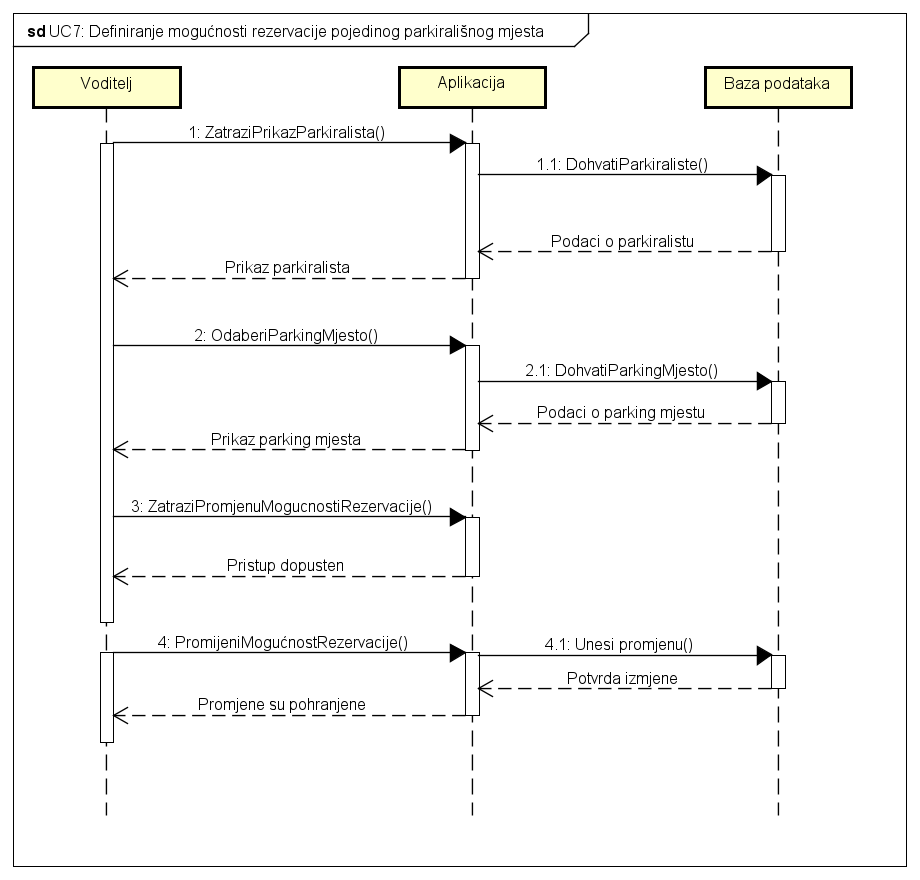
\includegraphics[width=\textwidth]{slike/MogucnostRezervacije.png} %veličina slike u odnosu na originalnu datoteku i pozicija slike
					\caption{Sekvencijski dijagram za UC7}
					\label{fig:mogucnostRezerv}
				\end{figure}
				\eject	
				
		\section{Ostali zahtjevi}
		
			\textbf{\textit{dio 1. revizije}}\\
		 
			 \textit{Nefunkcionalni zahtjevi i zahtjevi domene primjene dopunjuju funkcionalne zahtjeve. Oni opisuju \textbf{kako se sustav treba ponašati} i koja \textbf{ograničenja} treba poštivati (performanse, korisničko iskustvo, pouzdanost, standardi kvalitete, sigurnost...). Primjeri takvih zahtjeva u Vašem projektu mogu biti: podržani jezici korisničkog sučelja, vrijeme odziva, najveći mogući podržani broj korisnika, podržane web/mobilne platforme, razina zaštite (protokoli komunikacije, kriptiranje...)... Svaki takav zahtjev potrebno je navesti u jednoj ili dvije rečenice.}
			 
			 
			 
	